\documentclass[
	ngerman,
	ruledheaders=section,%Ebene bis zu der die Überschriften mit Linien abgetrennt werden, vgl. DEMO-TUDaPub
	class=report,% Basisdokumentenklasse. Wählt die Korrespondierende KOMA-Script Klasse
	thesis={type=master},% Dokumententyp Thesis, für Dissertationen siehe die Demo-Datei DEMO-TUDaPhd
	accentcolor=9c,% Auswahl der Akzentfarbe
	custommargins=true,% Ränder werden mithilfe von typearea automatisch berechnet
	marginpar=false,% Kopfzeile und Fußzeile erstrecken sich nicht über die Randnotizspalte
	%BCOR=5mm,%Bindekorrektur, falls notwendig
	parskip=half-,%Absatzkennzeichnung durch Abstand vgl. KOMA-Script
	fontsize=11pt,%Basisschriftgröße laut Corporate Design ist mit 9pt häufig zu klein
%	logofile=example-image, %Falls die Logo Dateien nicht vorliegen
]{tudapub}


% Der folgende Block ist nur bei pdfTeX auf Versionen vor April 2018 notwendig
\usepackage{iftex}
\ifPDFTeX
	\usepackage[utf8]{inputenc}%kompatibilität mit TeX Versionen vor April 2018
\fi

%%%%%%%%%%%%%%%%%%%
%Sprachanpassung & Verbesserte Trennregeln
%%%%%%%%%%%%%%%%%%%
\usepackage[english, main=ngerman]{babel}
\usepackage[autostyle]{csquotes}% Anführungszeichen vereinfacht

% Falls mit pdflatex kompiliert wird, wird microtype automatisch geladen, in diesem Fall muss diese Zeile entfernt werden, und falls weiter Optionen hinzugefügt werden sollen, muss dies über
% \PassOptionsToPackage{Optionen}{microtype}
% vor \documentclass hinzugefügt werden.
\usepackage{microtype}

%%%%%%%%%%%%%%%%%%%
%Literaturverzeichnis
%%%%%%%%%%%%%%%%%%%
\usepackage{biblatex}   % Literaturverzeichnis
\bibliography{DEMO-TUDaBibliography}


%%%%%%%%%%%%%%%%%%%
%Paketvorschläge Tabellen
%%%%%%%%%%%%%%%%%%%
%\usepackage{array}     % Basispaket für Tabellenkonfiguration, wird von den folgenden automatisch geladen
\usepackage{tabularx}   % Tabellen, die sich automatisch der Breite anpassen
%\usepackage{longtable} % Mehrseitige Tabellen
%\usepackage{xltabular} % Mehrseitige Tabellen mit anpassbarer Breite
\usepackage{booktabs}   % Verbesserte Möglichkeiten für Tabellenlayout über horizontale Linien

%%%%%%%%%%%%%%%%%%%
%Paketvorschläge Mathematik
%%%%%%%%%%%%%%%%%%%
%\usepackage{mathtools} % erweiterte Fassung von amsmath
%\usepackage{amssymb}   % erweiterter Zeichensatz
%\usepackage{siunitx}   % Einheiten

\usepackage{graphicx}
\graphicspath{ {../images/} }

%Formatierungen für Beispiele in diesem Dokument. Im Allgemeinen nicht notwendig!
\let\file\texttt
\let\code\texttt
\let\tbs\textbackslash
\let\pck\textsf
\let\cls\textsf

\usepackage{pifont}% Zapf-Dingbats Symbole
\newcommand*{\FeatureTrue}{\ding{52}}
\newcommand*{\FeatureFalse}{\ding{56}}

\begin{document}

\Metadata{
	title=TUDaThesis - Abschlussarbeiten im CD der TU Darmstadt,
	author=Linnea Widmayer
}

\title{TUDaThesis -- Abschlussarbeiten im CD der TU Darmstadt}
\subtitle{Subtitle}
\author[L. Widmayer]{Linnea Widmayer}%optionales Argument ist die Signatur,
%\birthplace{Geburtsort}%Geburtsort, bei Dissertationen zwingend notwendig
\reviewer{Nico Faul \and Prof. Thomas Burg}%Gutachter

%Diese Felder werden untereinander auf der Titelseite platziert.
%\department ist eine notwendige Angabe, siehe auch dem Abschnitt `Abweichung von den Vorgaben für die Titelseite'
\department{etit} % Das Kürzel wird automatisch ersetzt und als Studienfach gewählt, siehe Liste der Kürzel im Dokument.
\institute{Institut}
\group{Arbeitsgruppe}

\submissiondate{\today}
\examdate{\today}

% Hinweis zur Lizenz:
% TUDa-CI verwendet momentan die Lizenz CC BY-NC-ND 2.0 DE als Voreinstellung.
% Die TU Darmstadt hat jedoch die Empfehlung von dieser auf die liberalere
% CC BY 4.0 geändert. Diese erlaubt eine Verwendung bearbeiteter Versionen und
% die kommerzielle Nutzung.
% TUDa-CI wird im nächsten größeren Release ebenfalls diese Anpassung vornehmen.
% Aus diesem Grund wird empfohlen die Lizenz manuell auszuwählen.
%\tuprints{urn=XXXXX,printid=XXXX,year=2022,license=cc-by-4.0}
% To see further information on the license option in English, remove the license= key and pay attention to the warning & help message.

% \dedication{Für alle, die \TeX{} nutzen.}

\maketitle

\affidavit% oder \affidavit[digital] falls eine rein digitale Abgabe vorgesehen ist.
% Es gibt mit Version 3.20 die Möglichkeit ein Bild als Signatur einzubinden.
% TUDa-CI kann nicht garantieren, dass dies zulässig ist oder eine eigenhändige Unterschrift ersetzt.
% Dies ist durch Studierende vor der Verwendung abzuklären.
% Die Verwendung funktioniert so:
%\affidavit[signature-image={\includegraphics[width=\width,height=1cm]{example-image}}, <hier können andere Optionen wie z.B. affidavit=digital zusätzlich stehen>]

\tableofcontents

\chapter{Einleitung}
	% !TeX spellcheck = en_US

Light microscopy (LM) is the simplest and most commonly used to magnify small objects and structures. There are many building varieties for different applications with different magnification ranges. In general, two building variation exist: Transmission LM do let light pass trough the sample to create an image. Reflective LM uses the reflecting light from the sample for imaging. 

For example, some light microscopes have additional fluorescence filters to detect fluorescence signals. These filters allow only the specific wave length emitted by a fluorescent molecule to pass. As a light source, filtered white light and lasers can be used, since only a specific wavelength range excites fluorescent molecules.

In LM many new advancements are still made. The Abbe criterium is the major limit for many light microscopes. However, multiple modified LM methods exist which are able to increase the resolution beyond this limit \cite{Heintzmann.2006}.

Electron microscopy (EM) is another imaging method being used: With electrons, resolutions down to the size of atoms are possible. The smallest structures in sub nanometer scale are observable with this method. Even the distribution of certain elements is detectable. Also the creation of 3D images are possible.

In EM, water containing structures must be fixated. One way to archive fixation of the specimen is to freeze the water to ice at cryogenic temperatures. With rapid cooling below \SI{-120}{\degreeCelsius} within tenths of milliseconds, vitrified ice which is amorphic and does not destroy structures by forming ice crystals is reached  \cite{Wowk.2010}. This requires low thermal conductivity which is only achievable with small and well thermal conducting sample holders. To hold the ice structure, all setups including microscopes to handle the specimen needs to be cooled below \SI{-120}{\degreeCelsius} to prevent subsequent crystallization of the ice.

To reach transparency of the electron beam for cryo scanning electron microscopy (cryo-TEM), the sample is required to have a maximum thickness of \SI{100}{\nano\meter} and containing only lighter elements. Additionally, a thin film in combination of a metal grid is used as a sample holder \cite{Danino.2012}. This grid does not deliver a regular background. Additionally, the sample needs to have low absorption of light in the visible spectrum in case a laser being used. If the contrast is too high, the sample is damaged trough light absorption and resulting heat.

For cryo-LM, the thin ice layer is frozen onto a thin sapphire disk. also here the thickness is limited by thermal conductivity to reach the vitrified state. The surface needs to be transparent in visible light or with low contrast \cite{Faoro.2018}.

Conveniently, the process of sample preparation for cryo-LM and cryo-EM is very similar. Still, the sample holder used for LM and EM are very limited inter operable. This grid does not deliver a regular background for reflective EM. Also a grid is not completely transparent for light for transmissive LM. also the grid absorbs visible light, limiting the use of lasers. The slides used in LM are mostly too thick for EM. Sometimes heavier elements are used too. Additionally some form of metal grid must be added for EM. 


Nevertheless, combining LM and EM on the same sample brings big advantages: The larger scale of LM and the use of multiple wavelengths combined with fluorescence and high resolution on the same sample does make studying samples easier. In this master thesis, a method for using cryo lLM and cryo-EM on the same sample is examined. To make this possible, the sample must be transferred to different sample holders between cryo-LM and cryo-EM without destroying the sample. To achieve this, a layer between ice and sample holder is engineered to enable detachment and transfer to another sample holder (Fig. \ref{fig:layersingeneral}).

\begin{figure}[hbt!]
	\centering
	\input{../images/Zeichnung_Layers_in_general.pdf_tex}
	\caption{Depiction of a sample. The specimen is frozen inside the ice layer. The sample holder and ice layer are connected by an additional engineered layer. In this master thesis, the additional layer is varied to allow separation of the ice including the specimen from the sample holder.}
	\label{fig:layersingeneral}
\end{figure}


\section{Task and requirements}

There are several requirements for this engineered layer: The layer must be thin to keep thermal conductivity high at freezing. The layer also must be hydrophilic and even to  enable freezing a regular thin ice layer on top. The engineered layer should not disturb LM or EM. 

The order of which kind of microscopy is performed first has an influence on the design of the layer. As the thickness and the design of the sample holder is less restrictive at LM, designing the layer for this environment is also easier. Therefore, LM is performed first in the final process. Then the ice layer is transferred to a grid. After this, cryo-EM is performed.

There are several challenges to perform a sample holder change: First, high wettability is needed when plunge-freezing. Wettability highly increases adhesion of ice on the rest of the sample. Second, the engineered layer is thin and covered by ice and sample holder. Therefore access to the layer is limited by solvents or other liquids. Third, the ice layer must stay in a vitrified state in the whole process. Last, many characteristics are temperature dependent. Results of experiments done at room temperature or close to freezing point are not easily transferable at \SI{-140}{\degreeCelsius}. For example, even mechanical stability and adhesion forces of all layers varies over temperature. Therefore everything needs to be validated at cryogenic temperatures \cite{Makkonen.2012}.

To fulfill all the requirements, following ideas are pursued. A sacrificial layer between sample holder and ice could be dissolved. The ice layer will float separately in the solution and could then be transferred to another sample holder. The second idea is to mechanically separate a piece or the hole ice layer from the sample holder. The layer must be designed in a way to reduce adhesion and posses high wettability at the same time. Also the forces applied must be strong enough for separation.

%First, I investigated lipids for positive characteristics for usage as a sacrificial layer. Second, different layers are tested for low ice adhesion. Also different parameters on the mechanical setup are tested.

\section{State-of-the-art}
\label{section:Stateoftheart}

Ice removal is needed in multiple commercial applications. Most strategies are only applicable in temperatures down to \SI{-30}{\degreeCelsius}. Since the ice layer in the demonstrated application needs to stay vitrificated at under \SI{-140}{\degreeCelsius} or even lower, only few anti-frosting methods are feasible. For example the active anti-frosting strategy of heating the ice is not possible, as the specimen must stay contained within the ice layer.

There are four passive anti-frosing strategies: Inhibition of ice nucleation is achieved by using surface inherent properties to prevent ice crystals from forming. Retardation of frosting removes water to prevent icing on the surface with water repellent properties such as the lotus effect. Mitigation of frost accumulation prevents already formed ice droplets from further accumulating and forming an ice layer. Last a reduction of ice adhesion on the surface prevents ice droplets to stay on the surface. Other forces like wind or gravity removes ice droplets and keeps the surface ice free \cite{Yang.2021}. 

Out of the four passive anti-frosting strategies, only one is applicable at cryogenic temperatures. The reduction of ice adhesion can be used to decrease the force needed to separate the ice layer mechanically. This can be done by using a hydrophobic surface with general low adhesion or with surface structuring. In contrast, Inhibition of ice nucleation, retardation of frosting and mitigation of accumulation only inhibit the freezing process itself and are therefore not applicable.

In industrial application, one commonly used coating to reduce adhesion of ice is Polydimethylsiloxane (PDMS). PDMS is a polymer which is widely used in different applications like in fabrication of micro channels, chip manufacturing, aerospace industry and medical tools. PDMS properties are for example its hydrophobility, biocompatability and electric insulating capabilities. Also PDMS is cost effective and allows rapid prototyping, molding and thin coatings \cite{Wolf.2018}. Additionally, PDMS is modifiable with additives.

One example in which the low ice adhesion potential of PDMS is illustrated is the passive deicing of Aircrafts in flight. As ice can influence the air flow around the wing an the body, which induces turbulence and reduces lift. Ice protection is therefore critical for a save and stable flying. In \cite{Liu.2018}, PDMS is tuned for optimal characteristics in flight. To test the surfaces, flight conditions of \SI{0.5}{\bar} and \SI{-12}{\degreeCelsius} are simulated. Fluorinated PDMS with and without silica nanoparticles are compared to aluminum, showing better resistance against ice growth. The different coatings are also examined regarding contact angle of water and surface roughness. Also the stability of the surface is relevant as ice formation and impacts can also wear down the coating itself. 

To create PDMS surfaces in labs Dowsil Sylgard 184 Silicone elastomer is widely used\cite{DOW.}. The PDMS kit includes a curing agent and base coat component. The specified mixture ratio is 10 base coat to 1 curing agent in weight (10:1). In some applications, other mixture ratios are used and additives are added for tuning PDMS.

For example, adhesion forces of ice on PDMS varies with different mixture ratios. In \cite{IbanezIbanez.2022}, PDMS is investigated in 3:1 to 1:50 weight ratio. The mixture is given into a mold and afterwards fully cured. An ice block is frozen on top of the PDMS. Using a pulling machine the maximum tensile and shear forces for detaching ice from PDMS are determined. Results show that mixture ratios 10:1 to 1:3 have significant lower adhesion forces on ice. At for example at 2:1, the shear mode is just under \SI{20}{\kilo\pascal} and the tensile mode around \SI{30}{\kilo\pascal}. 

Plasma curing is commonly used as PDMS treatment. Plasma treatment used for increasing wettability and adhesion. Plasma treatment is changing the chemistry of the polymer chains on the surface. Charged Oxygen Ions are deposited on the surface. these Ions make the surface temporarily hydrophile and increasing water adhesion. The Ions change the structure of the PDMS is permanently by oxidation. In some cases, cracks form as the surface oxidizes to a silica like form.

In \cite{Owen.1994}, the influence of different gasses on PDMS plasma treatment are examined. Oxygen, Nitrogen, Argon and Helium are compared on the effect on wettability, adhesion and cracking. Thin PDMS sheets are used with unknown composition. They found similar results between gasses. All gasses produced a thin and brittle surface with cracks and high wettability. Based on these results, used gas is not a significant factor for plasma activation. Therefore using only air (mainly a mixture of nitrogen and oxygen) is sufficient to determine the effect of plasma treatment.

In \cite{Ohishi.2017}, the influence of plasma treatment on Mixture ratios of 50:1 to 100:1 is described. A thin layer of those PDMS mixtures is put onto a preformed PDMS piece with lower mixture ratio. The preformed piece is used to apply shear stress to the surface by stretching the lower PDMS form piece. Therefore only tensile force are examined. It shows no significant difference between described mixture ratios. It also shows that higher plasma treatment leads to more brittle surfaces, reducing the force needed to break the PDMS Layer by $90\,\%$.

PDMS properties are also temperature dependent. In \cite{Zhang.2020}, multiple characteristics are determined for cryogenic temperatures. The PDMS is prepared with the standard mixture ratio of 10:1. The compressive strength increases with lower temperatures until \SI{-123.15}{\degreeCelsius}. At this temperature, the compressive strength reaches a maximum of \SI{224.50}{\mega\pascal} in average. At lower temperatures, the PDMS gets brittle. At \SI{-150.15}{\degreeCelsius} PDMS has a compressive strength of \SI{106.99}{\mega\pascal}.

%&The effect of Plasma activation between mixture ratios is mostly unknown. At mixture ratios above 50:1 base coat to curing agent, no significant differences between plasma activation is observed \cite{Ohishi.2017}. 



\chapter{Methode}
	
\chapter{Ergebnisse}
	% !TeX spellcheck = en_US


\section{Lipids}

In the previous chapter, the method of using a sacrificial layer to detach Ice was discussed. For this, lipids need to be solved at cryogenic temperatures. As not every lipid is solvable the same way in different solvents, a first test is conducted to obtain the potential solvents at room temperature. then the best solvents are also tested at cryogenic temperatures.

The solubility of lipids at room temperature in different solvents are tested. For this experiment the cover glasses are coated with lipids. Then a first reference image was taken. Then the cover glass is given into a small container with the potential solvent. After 15 minutes, the cover glass is removed and compared under the microscope with the reference picture. If streaks created from lipids are still as visible as before, the lipids are categorized as insoluble in this solvent. If the streaks partially dissapeared and/or are less visible, the lipids are categorized as partially soluble in this solvent. Last if the streaks completely disappear, the lipids are assinged as soluble in the solvent (Table \ref{table:LoeslichkeitRaumtemperatur}).


\begin{table}[hbt!]
	\centering
	\begin{tabular}{|l|c|c|}
		\hline
		potential solvent & solubility EGG-PC & solubility DOPC \\
		\hline
		\hline
		4-Methyl Pentene & soluble & N/A  \\ 
		\hline
		3-Methyl Pentene & slightly soluble & insoluble \\
		\hline
		1-Pentene & insoluble & insoluble \\
		\hline
		Isopentane & soluble & slightly soluble\\
		\hline
		1-Propanol & soluble & soluble\\
		\hline
		Pentane & soluble & insoluble\\
		\hline
		Ethanol & N/A & soluble\\
		\hline
	\end{tabular}
	\caption{result of solubility tests at room temperature. soluble indicates solvents which are able to visibly solve all lipids off a cover glass. slightly soluble indicates solutions which are able to solve lipids, but some stains are left: insoluble indicates no visible changes of tested lipid.}
	\label{table:LoeslichkeitRaumtemperatur}
\end{table}

This experiment shows that three different solvent exist for each EGG-PC as well as DOPC with high solubility (Table \ref{table:LoeslichkeitRaumtemperatur}). Following those results, solvents categorized with "soluble" are tested regarding solubility at temperatures of \SI{-140}{\degreeCelsius}. As not all solutions are liquid at \SI{-140}{\degreeCelsius} (Table \ref{table:SchmelztemperaturLösungsmittel}), they are tested at higher temperatures above their melting point, as mentioned in chapter \ref{chapter:meltingtemp}. In addition they are tested as mixtures with other solvents with a lower melting point, to lower its melting point. Additionally all lipids are tested in liquid ethane. Ethane was not tested at room temperature, as the boiling point is at \SI{-88.6}{\degreeCelsius} (ZITAT PUBCHEM ETHANE).

This experiment shows that no tested solvent was able to completely solve lipids at \SI{-140}{\degreeCelsius} and within \SI{15}{\minute} (Table \ref{table:Cryoloeslichkeit}). Also the smears of lipids did not only stay partially behind, but also new streaks appear on the glass slides. This means that some lipids redistributed on the glass slide.

Using solvents to destroy a sacrificial layer, a high solubility is a requirement. In this case, the sacrificial layer would be completely covered by the ice layer except the edges. So the solvents have only a small area to start solving the layer. To solve it completely, a strong solvent is needed to detach the ice layer from the slide. Additionally, as the ice layer needs to stay vitrified, the temperature cannot be raised over \SI{-140}{\degreeCelsius}. 

The solving process of lipids in solutions is probably endothermic. This means that heat is needed to solve lipids, so cold temperature heavily decrease solubility QUELLE DENNIS ODER SO. This effect was observed over the last experiments by all solvents to varying degree. It can be assumed that the majority of solvent lipids mixtures are endothermic which is very disadvantageous for finding a potential solvent lipid candidate. Strongly exothermic solvents could heat up the ice enough to create ice crystals, which would not be feasible. So only weakly exothermic solvents are feasible for this task. 

\begin{table}[hbt!]
	\begin{subtable}{\linewidth}
		\centering
		\begin{tabular}{|l|l|}
		\hline
		Solvent & Result \\
		\hline
		\hline
		Pentane & soluble at \SI{-125}{\degreeCelsius} \\
		\hline
		4-methyl pentene & insoluble \\
		\hline
		\makecell[l]{1:1 volume ratio\\ HFE to 1-Propanol} & \makecell[l]{did not mix,\\ slightly soluble}\\
		\hline
		Liquid ethane & insoluble\\
		\hline
		\end{tabular}
		\caption{EGG-PC}
		\label{table:EGG-PCCryoloeslichkeit}
	\end{subtable}
	\begin{subtable}{\linewidth}
		\centering
		\begin{tabular}{|l|l|}
		\hline
		Solvent & Result \\
		\hline
		\hline
		\makecell[l]{1:4 volume ratio\\ 1:2 molar ratio\\ Ethanol to Isopentane} & slightly soluble\\
		\hline
		\makecell[l]{1:2 volume ratio\\ 1:1 molar ratio\\ 1-Propanol to Isopentane} & insoluble \\
		\hline
		Isopentane & slightly soluble\\
		\hline
		1-Propanol & \makecell[l]{at \SI{-130}{\degreeCelsius}\\ slightly soluble}\\
		\hline
		Liquid ethane & insoluble \\
		\hline
		\end{tabular}
		\caption{DOPC}
		\label{table:DOPCCryoloeslichkeit}
	\end{subtable}
	\caption{ in \ref{table:EGG-PCCryoloeslichkeit} for EGG-PC, no sufficient solubility at -140°C was found. In \ref{table:EGG-PCCryoloeslichkeit}, DOPC was tested but also no proper solution was found.}
	\label{table:Cryoloeslichkeit}
\end{table}

As finding a good solvent lipid combinations seems very unlikely, a new method was tested. In the next section, the finger tool is used to try mechanically detach the ice layer.

\FloatBarrier
\section{Finger}

For this section, cover glass coated in Parylene are used as object slide. The slide is then dipped in solution containing lipids for a lipid coating. A ice layer with fluoriscine is frozen with either plunge-freezing or using a pincer and liquid nitrogen. Additionally, the "finger" is used as tool to try lifting off a piece of ice from the frozen layer on top of the lipids. In the next sections, different variables are examined and tested.

\subsection{Finding right dosage of HFE}

First obvious variable and potential issue source is the amount of HFE used as glue. High dosages of liquid hfe can spread underneath the frame holding the sample, leading to an inefficient force distribution. Also a big glue layer is a weak point between finger and sample, leading to a reduction of maximum force which can be applied. Too little glue will not connect the finger to the sample. Additionally, the dosaging of glue revealed to be a big challenge.

The HFE is dosaged with a pipette. The HFE is "taken up WORD" at room temperature, then the HFE is "released WORD" on the tip of the finger. In between, HFE is evaporating. Around $4\,\mu l$ is evaporating each time. Based on this knowledge, dosaging $4.10\,\mu l$, $4.30\,\mu l$ and $4.50\,\mu l$ is compared and a picture is made.

Results show that pipetting HFE is not reliable. The range spreads of too little to too much HFE even for those dosages. Not only differences in evaporation are playing a role. Correct placement on the tip is a major factor of glue dosaging. Still, a visual estimate for the correct glue dosage can be made by calculating the drop volume out of camera images.

\begin{figure}[hbt!]
	\centering
	\begin{subfigure}[]{0.45\textwidth}
		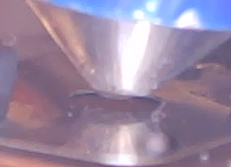
\includegraphics[width=6cm]{Temp_Picture_Lower_Limit}
		\caption{chosen example for lower limit}
	\end{subfigure}
	\begin{subfigure}[]{0.45\textwidth}
		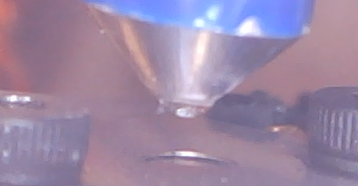
\includegraphics[width=6cm]{Temp_Picture_Upper_Limit}
		\caption{chosen example upper limit}
	\end{subfigure}
	\caption{example of upper limit and lower limit for glue dosages. (BETTER PICTURES NEEDED)}
\end{figure}

To calculate the actual glue dosage, two exemplary Pictures of an Upper and lower limit of glue dosages is picked. Then the Volume is calculated with a formula for the volume of a spherical section. All needed components are calculated out of the estimated contact angle of the glue $\alpha \approx 45°$ and the tip diameter of $d = 1.68\,mm$, for the lower range a reduction of $d$ by a factor of $\frac{2}{3}$ is assumed as the drop is not covering the whole tip. The resulting volume range of the glue dosage is $ 0.11\,\mu l \gtrapprox V \gtrapprox 0.38\,\mu l $. Also the lower end of this range is desired, but the repetition range in correctly dosaging lower doses is lower.

\subsection{Temperature over applied force}

As the HFE gluing effect is temperature dependent, the temperature needs to be regulated precisely. To narrow in the temperature dependency of HFE, the properties of HFE are observed at different temperatures in a regulated bath. Between -160°C and -170°C, the HFE is increasingly viscious. Under this temperature, HFE Freezes and gets brittle. Over this temperature range, HFE is too fluid to transfer any tensile forces. 

In application tests on lipid samples, the temperatures -160°C, -165°C and -170°C are compared. It was observed that decreasing temperatures lead to higher forces transferred to the sample. At the same time, temperatures are not reliably reached under -160°C.
As lower temperatures leads to an additional factor for repeatability issues, -160°C is used all other experiments.

\subsection{Tensile mode vs Shear mode}



\subsection{Detaching ice with finger of plunge freezed samples}

Next observed possible factor is the thickness of the ice layer. In the following, samples freezed with a plunge-freezer are compared to samples freezed with a pincer in liquid nitrogen. The results are categorized in 4 categories: Not successful pulls don't have visible changes of the flourescent ice layer, Partially successes are visible breaks or clear movement of ice parts on the ice layer, Successful liftoff is a missing piece and a visible piece on the finger, which could be used for future steps. In the results, there is no difference between Hand freezed and plunge-freezed samples regarding detachability. Therefore Ice thickness is not a factor which makes detaching ice easier. As both methods don't show success in detaching ice pieces, it could still be a relevant factor but not a thing which should make a certain solution magically work xD

\subsection{other observed error sources??}

Wrong positioning, forming of ice

\begin{table}
	\centering
	\begin{tabular}{|c|c|c|}
		\hline
		Category & Hand-freezed & Plunge-freezed \\
		\hline
		\hline
		count executed tries & 4 & 4\\
		\hline
		unsuccessful & 3 & 3\\
		\hline
		breaks/movement of ice & 1 & 1\\
		\hline
		piece lifted with finger & 0 & 0\\
		\hline		
	\end{tabular}
	\caption{Comparison of detachability between hand-freezed and plunge-freezed samples}
\end{table}

\section{PDMS}

Now two mixture ratios of PDMS are compared. For this, samples where coated with 4:1 and 1:2 curing agent to base coat weight ratio. Also for ..., glass without pdms is used. The pulling mashine was used to determine the max force. A plexiglass stamp was used for pulling off the PDMS layer. UV Glue was used to fixate the plexiglass onto the PDMS and is cured with 3 min UV exposure. After pulling, the Area of the separating layers is determined via microscope. Then the max pulling tension is calculated. This was repeated several times. The Result shows, that glass is hardest do pull off. Then 4:1 is harder to separate than 1:2 (Fig. \ref{fig:vgl4:1zu1:2zuGlas}). In literature, 1:2 weight ratio should have a lower adhesion force on ice too\cite{IbanezIbanez.2022}. For those reasons, 1:2 was picked to continue experiments with plasma treatment.

\begin{figure}
	\centering
	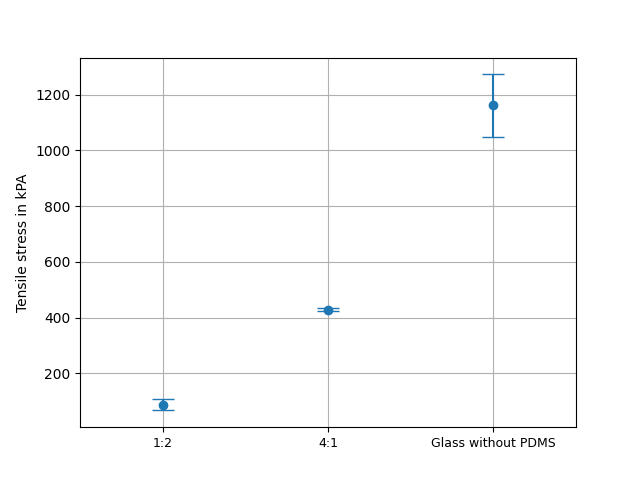
\includegraphics[width=14cm]{plotVGLZugspannungPDMSMischungsverhaeltnisse}
	\caption{Comparison 4:1, 1:2 Base coat to curing Agent and glass without PDMS}
	\label{fig:vgl4:1zu1:2zuGlas}
\end{figure}

\begin{figure}
	\centering
	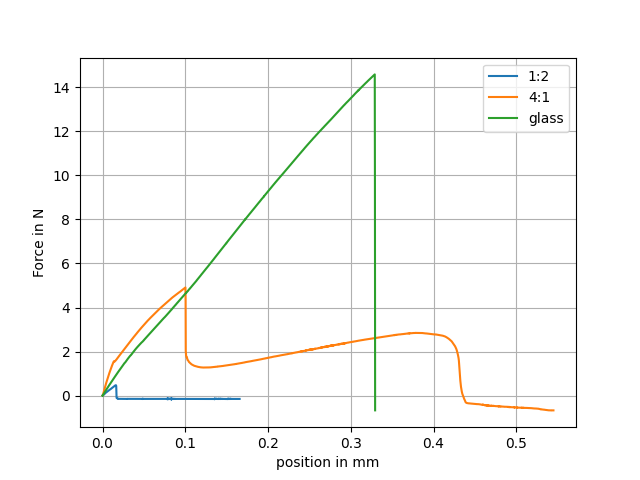
\includegraphics[width=14cm]{ForceOverTime}
	\caption{force over Time}
\end{figure}

In the next experiment, the effect of plasma curing is investigated. The same setup is used. Samples with a 2:1 weight ratio are additionally plasma treated before quickly clamping on the pulling mashine. Even with low repetition rates, a clear tendency can be observed. With lower and stronger plasma treatment, the durable the PDMS Layer gets (Fig. \ref{fig:PlotPlasmaAktivierung}). Over the whole range, The needed stress sextubles. Because the repititon rate is low, the exact values should be treated cautiosly. Also the results are not applicable to other mixture ratios, as different behaviour in plasma activation was observed between 2:1 and 4:1 weight ratio. also no glass-like state was observed in 2:1 weight ratio mixture.


\begin{figure}[h]
	\centering
	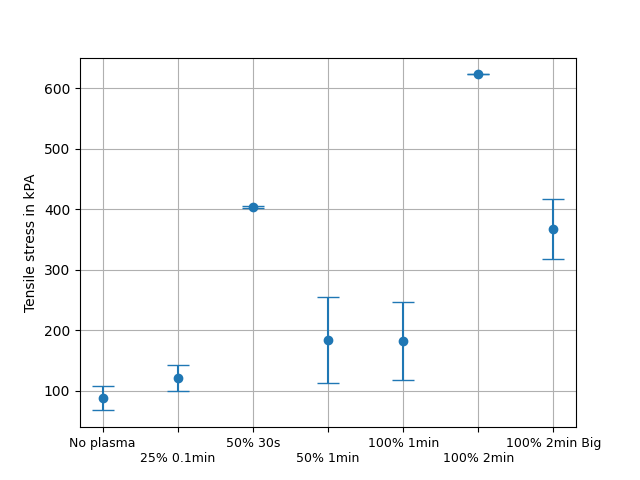
\includegraphics[width=14cm]{plot2_1PlasmaAktivierung}
	\caption{PDMS 2:1 Comparison between various Plasma curing strengths and durations.}
	\label{fig:PlotPlasmaAktivierung}
\end{figure}




\chapter{Diskussion}
\chapter{Zusammenfassung}
\chapter{Schluss}

\chapter{Quellen}
\printbibliography

\end{document}
